% !TeX encoding = UTF-8
% !TeX root = ../main.tex
\chapter{Implementácia vzorovej sady grafických komponentov}

\section{Príklad vytvorenia prečerpávacej stanice v Inkscape}

Nakreslenie jednotlivých častí komponentov prečerpávacej stanice v Inkscape bolo realizované pomocou ľavého bočného panela. Prečerpávacia stanica sa skladá z potrubí, indikátora úrovne hladiny vody, motora, a dvoch symbolov prítoku hladiny. Ako je možné vidieť na obrázku  \ref{picture1}.  


\begin{figure}[H]
	\begin{center}
		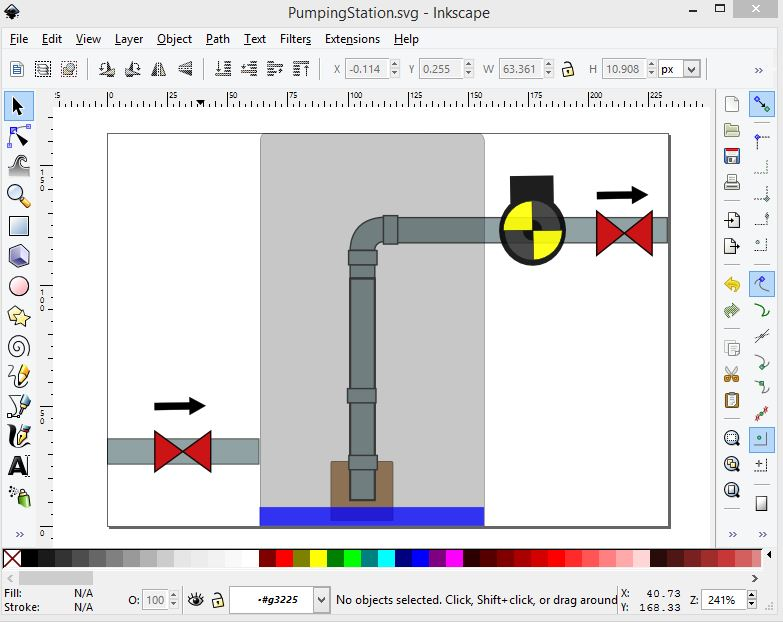
\includegraphics[width=0.7\linewidth] {obrazky/pump1.jpg}
		\caption{Grafické prostredie programu Inkscape s nakreslenou prečerpávacou stanicou}
		\label{picture1}
	\end{center}
\end{figure}


\section{Definovanie id v SVG}

Pre ovládanie JavaScriptom je nutné si pozrieť jednotlivé jedinečné identifikačné názvy. V .svg súboroch sú označované ako id. V zdrojovom kóde .svg súboru je to označené id="nazovElementu". Na ovládanie časti svg elementu v JavaScripte bude realizované cez CSS selektor, kde pristúpim k id svg cez značku \#.  Napríklad: paper.select("\#ventil"); .


\subsection{Object Properties}
Zistenie id je pomerne jednoduché v Inkscape. Klikneme pravým tlačidlom na daný komponent, ktorého id chceme vedieť, a potom na Objekt Properties.

Po kliknutí sa nám zobrazí okno s názvom Object Properties. 

\begin{figure}[H]
	\begin{center}
		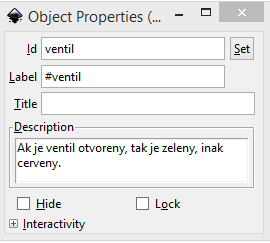
\includegraphics [width=5cm]  {obrazky/obr3.png}
		\caption{Object Properties}
		\label{picture3}
	\end{center}
\end{figure}


Z obrázka č.\ref{picture3} možno vyčítať aké je ID, predvolené sú tam napríklad desc3072. Hodnoty je možné prepísať a zmeniť stlačením tlačidla Set. Pre nás je dôležitá hodnota v kolónke id - ventil. 

V okne Object Properties je možné nastaviť script na animovanie. Po kliknutí na Interactivity sa zobrazia ďalšie kolónky, kde je možné zadať akciu, ktorá má nastať.  


\subsection{XML Editor}
Ďalší spôsob získania informácii o svg cez Inkscape je cez zabudovaný XML Editor.
Stlačením klávesovej skratky SHIFT + CTRL + X, alebo v hornej lište v menu vybrať ponuku Edit a na spodku je XML Editor. Následne sa zobrazí okno, ktoré je na obrázku \ref{xmlEditor}.
\begin{figure}[H]
	\begin{center}
		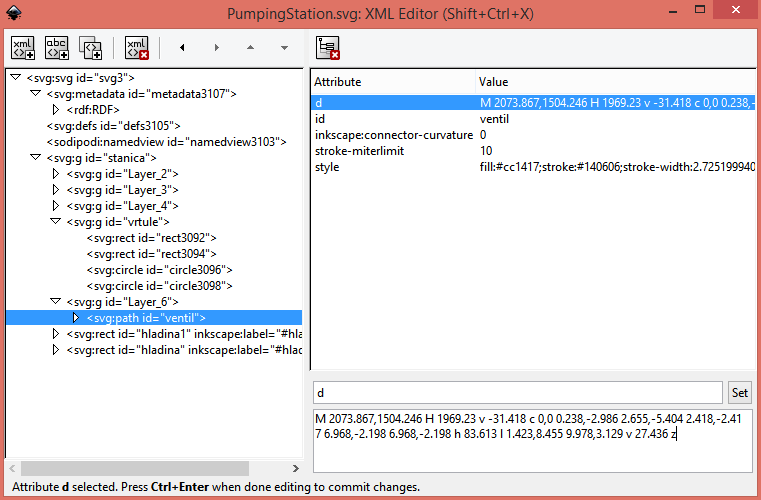
\includegraphics[width=0.6\linewidth]  {obrazky/XmlEditor2.png}
		\caption{Xml Editor v Inkscape}
		\label{xmlEditor}
	\end{center}
\end{figure}

XML Editor umožní zistiť ID jednotlivých komponentov, ale i hodnoty atribútov. 


\section{Integrácia prečerpávacej stanice pre dynamické ovládanie SVG objektu}

Súborová štruktúra prečerpávacej stanice: 
\begin{itemize}
	\item index.html 
	\item PumpingStation.js
	\item PumpingStation.svg
	\item TestPumpingStation.js
\end{itemize}

\subsection{HTML súbor}
Do HTML súboru index.html pridáme párový tag $<$svg$>$.  Na toto miesto sa neskôr vykreslí SVG načítané zo súboru cez JavaScript. Môže sa tu uviesť i celý kód SVG obrázka. V prípade, že nebude v dokumente dané kde presne sa nachádza SVG tag tak sa pridá na najbližšie voľné miesto. 
\subsection{Kód}
\begin{lstlisting}
<svg 
	id="svgStanica" 
	viewBox="0 0 750 600" 
	width="40%" 
	height="40%"> 
</svg>
\end{lstlisting}

\subsection{Vysvetlenie kódu}
Atribúty v tagu sú prispôsobené na to, aby sa grafický element vykreslil responzívne na obrazovku.
\begin{itemize}
\item  \textbf{id} - jedinečný identifikátor, cez ktorý meníme vlastnosti.
\item 	\textbf{viewBox} - je virtuálne okno, ktorým sa užívateľ uvidí svg obrázok. Je atribút, ktorý povoľuje špecifikovať danú množinu grafických komponentov, aby sa zobrazili v daných súradniciach x, y a šírke, výške. Hodnoty atribútov v viewBox sú štyri čísla - min-x, min-y, width a height. 
\item 	\textbf{width} a \textbf{height} je šírka a výška. Hodnoty atribútov je možné uviesť relatívne v percentách, alebo absolútne v pixloch. 
\end{itemize}

Do HTML dokumentu sa pridajú jednotlivé JavaScriptové knižnice s ktoré bude daný grafický komponent používať. 
\begin{lstlisting}[language = HTML]
<script type="text/javascript" src="../js/snap.svg-min.js">
</script>
<script type="text/javascript" src="PumpingStation.js">
</script>
\end{lstlisting}

Musíme sa uistiť, aby sa načítali všetky JavaScriptové knižnice, pred spustením funkcií. To zabezpečíme pridaním  onload do tagu $<$body$>$. 
\begin{lstlisting}
	<body onload="onPageLoad();">
\end{lstlisting}



\section{PumpingStation.js}
V súbore PumpingStation.js sú metódy na vizualizáciu grafického komponentu. V tejto časti je popis jednotlivých funkcií. 
Interface prečerpávacej stanice: 
\begin{itemize}
	\item onPageLoad();
	\item PumpingStation(nazovFileSVG, idDOMsvgElement);
    \item openValve1(isOpenValve1);
    \item animateTank(intPercent);
    \item rotateEngine(isRotating);
    \item openValve2(isOpenValve2);
    \item updateSchema01(isOpenValve1, intPercent, isRotating, isOpenValve2);
    \item updateSchema(updateData);
\end{itemize}

\subsection{onPageLoad()}
onPageLoad() sa spustí pri načítaní tela HTML súboru index.html. Následne spustí  PumpingStation(par1,, par2). Prvý parameter je udaný svg súbor vytvorení programom Inkscape. Druhý parameter je id tagu svg, kde sa vykreslí prečerpávacia stanica.

\begin{lstlisting}
function onPageLoad() {
	PumpingStation("PumpingStation.svg", "#svgStanica" );
}
\end{lstlisting}

\subsection{PumpingStation(par1, par2)}

Parametre pre PumpingStation sú názov svg súboru, a id, ktoré sa nachádza v tagu $<$svg$>$ html súbore.

Vo vnútri PumpingStation sa nachádza inicializácia globálnych atribútov. 
\begin{lstlisting}
var paper;
var idValve, idValve1 idNadrz, idHladina, idEngineMotor;

function PumpingStation(nazovFileSVG, idDOMsvgElement) {
	paper = Snap(idDOMsvgElement);
	Snap.load(nazovFileSVG, function (f) {
		idHladina = "#hladina";
		idNadrz = "#nadrz";
		idValve = "#ventil";
		idValve2 = "#ventil2";
		idEngineMotor = "#engineMotor";
		paper.append(f);
	});
}
\end{lstlisting}

Atribút paper je globálna premenná cez ktorú sa bude pristupovať k metódam JavaScriptovej knižnice Snap.svg. Jej parameter je referencia na plochu, kde bude vykreslené SVG elementy.

Vo vnútri funkcie volám z Snap.svg API funkciu load(). Má parametre názov súboru, a funkciu, ktorú spustí následne po načítaní. 
Vo vnútri funkcie load() sa inicializujú globálne premenné.  
Premenné obsahujú CSS selektor id získaný z programu Inkscape. Premenné budú slúžiť ako parameter pri volaní funkcie paper.select(). Pre prípadné zmeny v id, sa dané id zmení na jednom mieste a nemusí sa prepisovať všade. 

Význam premenných je nasledový: 
\begin{itemize}
	\item idHladina - indikátor prítoku hladiny vody, 
	\item idNadrz - je miesto, kde bude prichádzať prítok vody,
	\item idValve1, idValve2 - je ventil, 
	\item idEngineMotor - je symbol rotora motora.
\end{itemize}

Načítaný .svg súbor sa zobrazí volaním metódy append. 

\subsection{animateTank(percento)}
V tejto metóde je zobrazená vizualizácia prítoku hladiny do nádrže. Ako parameter slúži percento vyplnenia. 

\begin{lstlisting}
function animateTank(percento){
	var height = paper.select(idNadrz).getBBox().height;
	var y = paper.select(idNadrz).getBBox().y;
	var newHeight = height * (percento/100);
	var newY = y + height - newHeight;
	
	paper.select(idHladina).animate({
	y: newY,
	height: newHeight
	}, 1000);
}
\end{lstlisting}

Animovanie je realizované cez metódu animate zo Snap.svg API. 
Význam lokálnych premenných: 
\begin{itemize}
	\item height - výška nádrže do, ktorej bude pritekať voda,  získaná volaním metódy getBBox(),
	\item y - súradnica y - navýšením, alebo znížením hladiny sa mení súradnica y, a x zostava nezmenená,
	\item newHeight - vypočítaná nová výška hladiny podľa daného percenta, 
	\item newY - je vypočítaná súradnica - osi y. 
\end{itemize}

Volaním metódy animate, sa zanimuje daný element, v tomto prípade to bude hladina nádrže. Metóda má nasledovné parametre: \begin{itemize}
	\item atribúty - v pároch udané atribúty, ktoré sa zmenia. Zmení sa iba výška a os y, ostatné atribúty zostávajú nezmenené.
	\item rýchlosť animácie udaná v milisekundách. 
\end{itemize}

 
\subsection{openValve1(isOpen)}
Indikátor prítoku hladiny do prečerpávacej stanice je ventil, ktorý mení farbu. Ak je nastavený parameter isOpen na true, tak farba ventila bude zelená, v inom prípade červená. 
Zmena farby je realizovaná volaním metódy attr zo Snap.svg API, ktorá nastavila atribút fill daného elementu na danú farbu. Farba zmeny je zapísaná termálnym operátorom. 
Pre zmenu farby v druhom elemente je zápis identický až na to, že je zmena pri volaní select - na idValve2. 
\begin{lstlisting}
function openValve1(isOpen){
	paper.select(idValve).attr({
	fill: ((isOpen === "true") ?   "green" : "red")
	});
}
\end{lstlisting}



\subsection{rotateEngine(isRotating)}
Táto metóda bude rotovať až dovtedy pokým sa nezmení parameter isPaused. Rotácia motora je zabezpečená vnorenou metódou rotateLeft. Tá sa volá v toggleRotation(), kde v má parameter element vrtuliek čerpadla. 

Popis metódy rotateLeft():
\begin{itemize}
\item animationRunning - nastavené na true, znamená to, že animácia ešte beží
\item stringT0 - je transformačný string - potrebný na rotáciu vrtuliek čerpadla. Uhol rotácie je nulový, a súradnice stredovej osi x, y sú získané volaním metódy elementu getBBox().cx a getBBox().cy. 
\item transform() - je metóda z Snap.svg knižnice, ktorá umožní nastaviť transformáciu rotácie, kde parametrom je transformančný string. 
\item if(!(isPaused)){..} - je podiemka, ktorá zaručí opakované rotovanie elementu. 
\item stringT360 - je transformačný string, ktorý zrotuje element o uhol 360 stupňov zo stredom súradnicovej osi elementu. 
\item animate() - je metóda, kde animujem transformáciu z uhlu 0 stupňov na 360 stupňov. Ako parametre sú:
\subitem - párový atribút transform s hodnotou transformačného stringu, 
\subitem - rýchlosť animácie v milisekundách - 2000 ms, 
\subitem - mina objekt, ktorý zaručí lineárny plynulý pohyb, 
\subitem - callback funkcia, ktorá sa spustí po dokončení animácie. Toto zabezpečí opakované spustenie animácie rotácie elementu. 
\item else - ak skončí animácia - tak sa nastaví animationRunning na hodnotu false. 
\end{itemize}

\subsubsection{Kód metódy} 
\begin{lstlisting}
var isPaused = true;
var animationRunning = false;
function rotateEngine(isRotating){
	isPaused = isRotating;

	function toggleRotation() {
		if (!animationRunning && isPaused) {
			isPaused = false;
			rotateLeft(paper.select(idEngineMotor));
		} else {
			isPaused = true;}
	}
	toggleRotation();

	function rotateLeft(element) {
		animationRunning = true;
		var stringT0 = "R0,"+ element.getBBox().cx 	+ ","+
		element.getBBox().cy;
		element.transform(stringT0);

	if (!(isPaused)) {
		var stringT360 = "R360,"+ element.getBBox().cx 	+ ","+
		element.getBBox().cy;
		element.animate({
		 transform: stringT360 },
		 2000, 
		 mina.linear, 
		 rotateLeft.bind(null, element));
		} else { animationRunning = false;}
	}
}
\end{lstlisting}


%%%%%%%%%%%%%%%%%%%%%%%%%%%%%%%%%%%%%%%%%%%%%%%%%%%%%%%%%%%%%%%%%%%%%%%%%%%%%%%%%%%%%%%%%%%%%%%%%%%%%%%%%%%%%%%%%%%%%%%%%%%%%%%%%%%
\section{updateSchema()}

Metóda updateSchema01 zabezpečí aktualizáciu grafického komponentu. Parametre má nasledovné: 
\begin{itemize}
\item isOpenValve - boolean hodnota, ktorá nastaví indikátor prítoku vody, v prípade true - na zelený, v opačnom na červený. 
\item intPercento - je integer hodnota v rozsahu od 0-100. Vyjadruje percentuálne naplnenie nádrže. 
\item isRotating - boolean hodnota, ktorá nastaví otáčanie motora, až pokým sa znova nezavolá. 
\item isOpenValve - boolean hodnota druhého ventila. 
	
\end{itemize}

\begin{lstlisting}
function updateSchema01(isOpenValve1, intPercent, isRotating, isOpenValve2) {
	openValve1(isOpenValve1) ;
	animateTank(intPercent);
	rotateEngine(isRotating);
	openValve2(isOpenValve2);
}
\end{lstlisting}

Dáta vyjadrené vo formáte \ac*{JSON}. Zároveň je to interfejsná metóda k grafickému komponentu Pumping Station. Toto je príklad objektu update dátami na nastavenie hladiny nádrže na 20 percent a s ventilami, a rotorom zapnutým.  
\begin{lstlisting}
var updateData = {
	"valve1": "true",
	"tank": "20",
	"engineRotation": "true",
	"valve2": "true"
};
\end{lstlisting}
Metóda updateSchema s parametrom objekt updateData, aktualizuje grafický komponent na dané hodnoty. Zároveň je  to interfejsná metóda k REST API prečerpávacej stanice. Na obrázku \ref{fig:updateSchema} je zobrazený animovaný komponent s vopred pripravenými dátami. 
\begin{lstlisting}
function updateSchema(updateData){
	updateSchema01(updateData.valve1, updateData.tank, updateData.engineRotation, updateData.valve2);
}
\end{lstlisting}


\begin{figure}[H]
\centering
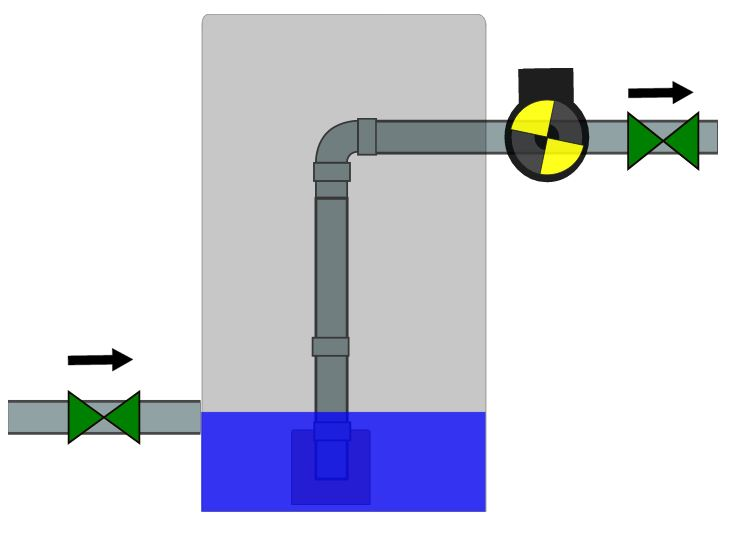
\includegraphics[width=0.7\linewidth]{obrazky/updateSchema}
\caption{Prečerpávacia stanica po vykonaní príkazu updateSchema(updateSchema);}
\label{fig:updateSchema}
\end{figure}





\section{Vzorová sada}
Vzorová sada grafických komponentov SCADA systémov obsahuje:
\begin{itemize}
	\item Prečerpávacia stanica - obrázok \ref{fig:pump}
	\item Prepravný pás - obrázok \ref{fig:belt}
	\item Trojcestný ventil - obrázok \ref{fig:trippleValve}
	\item Mapa Slovenska - obrázok \ref{fig:map}
	\item Thermometer - obrázok \ref{fig:thermometer}
\end{itemize}

Diagram tried vzorovej sady je na obrázku \ref{fig:classD} . 


\begin{figure}[H]
	\centering
	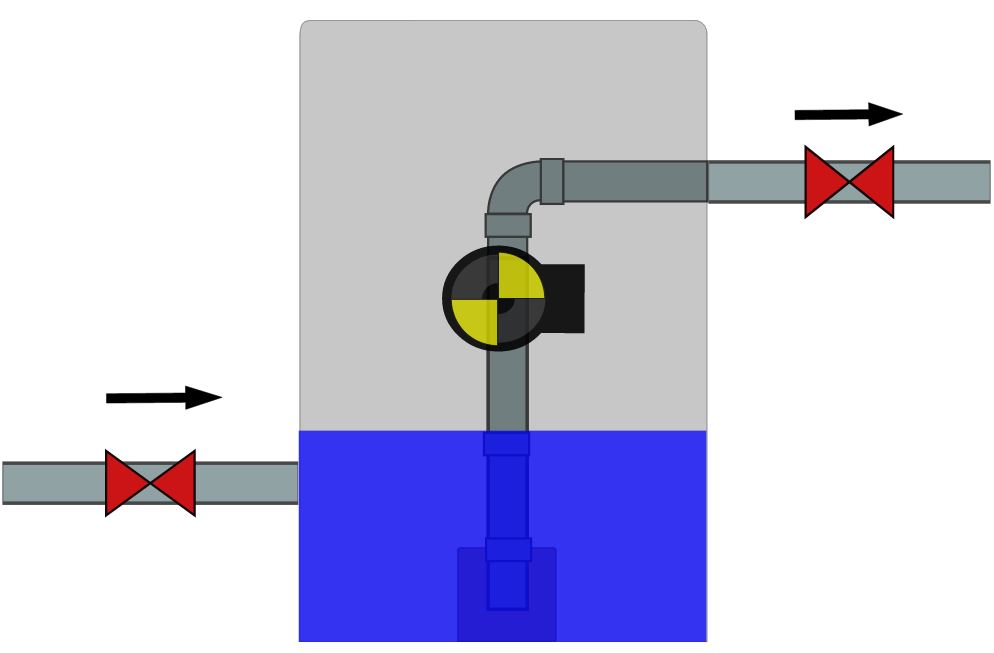
\includegraphics[width=0.7\linewidth]{obrazky/pump}
	\caption{Prečerpávacia stanica}
	\label{fig:pump}
\end{figure}
%%%%%%%%%%%%%%%%%%%%%%%%%%%%%%%%%%%%%%%%%%%%%%%%%%%
\begin{figure}[H]
	\centering
	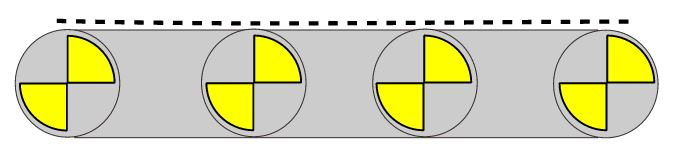
\includegraphics[width=0.7\linewidth]{obrazky/belt}
	\caption{Prepravný pás}
	\label{fig:belt}
\end{figure}
%%%%%%%%%%%%%%%%%%%%%%%%%%%%%%%%%
\begin{figure}[H]
	\centering
	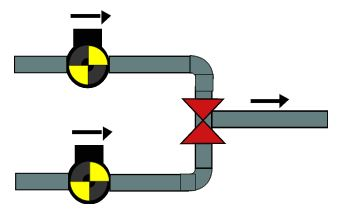
\includegraphics[width=0.7\linewidth]{obrazky/trippleValve}
	\caption{Trojcestný ventil}
	\label{fig:trippleValve}
\end{figure}
%%%%%%%%%%%%%%%%%%%%%%%%%%%%%%%%%%%%%%%%%
\begin{figure}[H]
	\centering
	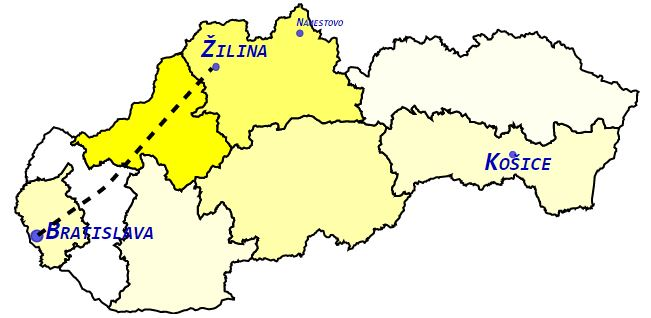
\includegraphics[width=0.7\linewidth]{obrazky/map}
	\caption{Mapa Slovenska}
	\label{fig:map}
\end{figure}
%%%%%%%%%%%%%%%%%%%%%%%%%%%%%%%%%%%%%%%%%%



%%%%%%%%%%%%%%%%%%%%%%%%%%%%%%%%%%%%%%%%%%%%
%%%%%%%%%%%%%%%%%%%%%%%
\begin{figure}[H]
	\centering
	
\includegraphics{obrazky/thermometer}
	\caption{Termometer}
	\label{fig:thermometer}
\end{figure}



\begin{figure}[hp]
\centering
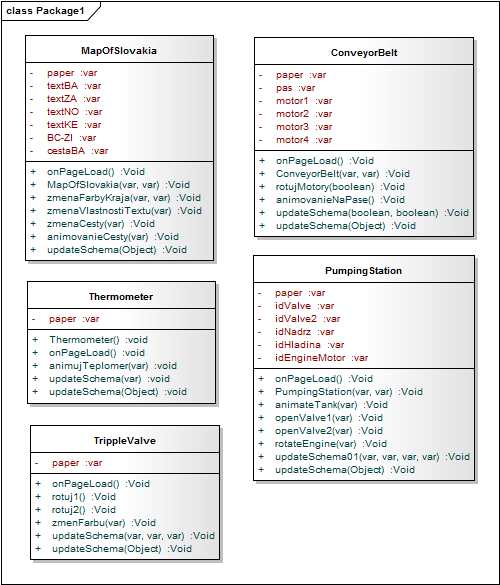
\includegraphics[width=1\linewidth]{uml/classDiagramTried}
\caption{Diagram tried vzorovej sady grafických komponetov}
\label{fig:classD}
\end{figure}
